\section{算法实现与结果分析}

\label{analize}

第\ref{analize}章将对以上提到的算法和改进进行实证研究,以评估算法的效率和改进方案。\ref{analize_subsection_1}节将介绍实验中使用的数据集、查询参数以及实验平台。4.2节将评估基于密度k-STC查询的改进方案。

\subsection{实验环境}
\label{analize_subsection_1}

本章的数据集来自网站kaggle上188593组餐厅信息,每组信息包括店铺ID,地理位置以及菜单信息。每家餐厅的文字描述长度平均为8个单词。具体来说,我们将18万组数据生成了大小为10k,50k,100k,150k,180k的数据集。利用不同的数据集测试算法性能。在180k的数据集中

在180k的数据集中随机选择一个对象p,利用位置偏离得到一个新的对象,新的对象文本描述保持一致。从对象的文本中随机选取单词作为查询关键字,关键词数量为1,2,3。因为查询集是对象文本的子集,所以不会有查询为空的情况。

实验评估了基本方法(basic)、带权重的IR-树的优化方法(Adv)。表\ref{args_scale}显示了实验中使用的参数值,其中粗体值是默认值。所有算法均采用Java语言实现,实验采用Intel(R) Core(TM) i5-4590 CPU @ 3.30GHz,内存8GB。所有的数据结构都保存在内存中。实验记录k-STC查询所需的平均运行时间。

\begin{table}[h!]
  \begin{center}
    \renewcommand\arraystretch{1.5}
    \begin{tabular}{|c|c|c|}
      \hline
      描述 & 参数 & 取值 \\
      \hline
      请求集群数 & $\left|q.\psi \right|$ & $1,2,3$ \\
      \hline
      \multirow{2}*{密度约束} & \varepsilon & $1,2,10,20,50$  \\
      \cline{2-3}
      ~ & $minpts$ & 1$0, 20, 50, 100$ \\
      \hline
      平均参数 &  $\alpha$ & $0.1, 0.3, 0.5, 0.7, 0.9$ \\
      \hline
      数据集大小 &$ \left| D \right|$ & $10k, 50k, 100k, 150k, 180k$ \\
      \hline
    \end{tabular}
    \caption{参数取值}
    \label{args_scale}
  \end{center}
\end{table}

\subsection{效果评估}
在不同参数设置不同的情况下,评估BASIC算法和改进方法。

\textbf{1. 改变关键词的数量$\left| q.\psi \right|$}

图\ref{change_key_num}显示了BASIC算法法和改进方法在改变查询关键字数量时的性能。关键词数量从1增加到3,随着查询关键字数量的增加,空间中相关的对象就越多,需要检查的簇就越多以及簇的范围就越大。搜索空间的加大直接影响了算法的性能,但因为优化方法可以更快地停止检查,所以始终比BASIC算法表现要好。

\begin{figure}[htbp]
  % caption放上面就会显示在图的上方,出现在下面就是出现在图的下方
  % label的位置也有讲究
  \begin{center}
    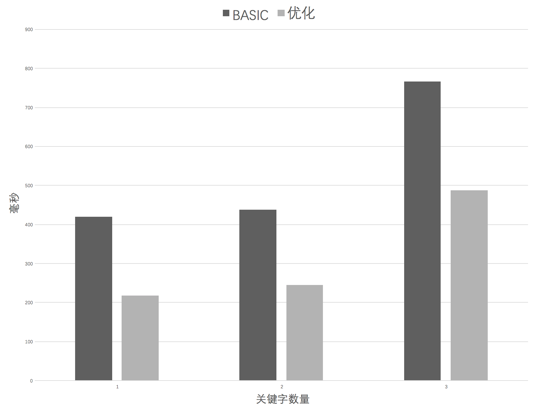
\includegraphics[width=4in]{barchart-about-keynum.png}
    \caption{改变关键词数量}
    \label{change_key_num}
  \end{center}
\end{figure}

\textbf{2. 改变密度约束}

密度要求包括两个参数, $\epsilon$ 和$minpts$。图\ref{change_epsilon}显示了BASIC算法和改进方法在不同$\epsilon$下的性能。图\ref{change_minpts}显示了它们在不同$minpts$时的性能,y轴取对数。$\epsilon$数值大或$minpts$数值小表明低密度的要求。随着$\epsilon$增加,性能变得更糟。原因是在保持$minpts$不变的前提下,邻域范围的扩大意味着该邻域内所包含的对象将增多,直接导致满足密度要求的簇将增多,这显然会带来更多的计算量,性能就会下降。然而,$minpts$在[10,100]的区间内,对性能影响并不明显。主要是因为在这个区间内,当邻域范围不变时,大多数的簇都远远大于密度要求,因此提高$minpts$不会带来显著的计算量增长,对性能的影响也就不明显了。

\begin{figure}[htbp]
  % caption放上面就会显示在图的上方,出现在下面就是出现在图的下方
  % label的位置也有讲究
  \begin{center}
    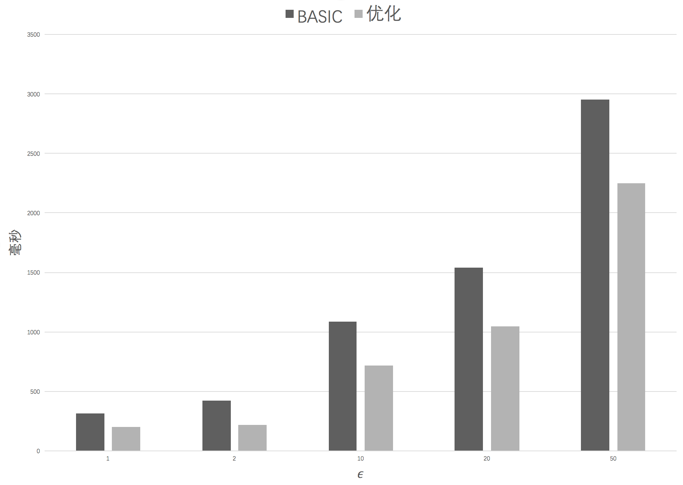
\includegraphics[width=4in]{barchart-change-e.png}
    \caption{改变$\epsilon$}
    \label{change_epsilon}
  \end{center}
\end{figure} 


\begin{figure}[htbp]
  % caption放上面就会显示在图的上方,出现在下面就是出现在图的下方
  % label的位置也有讲究
  \begin{center}
    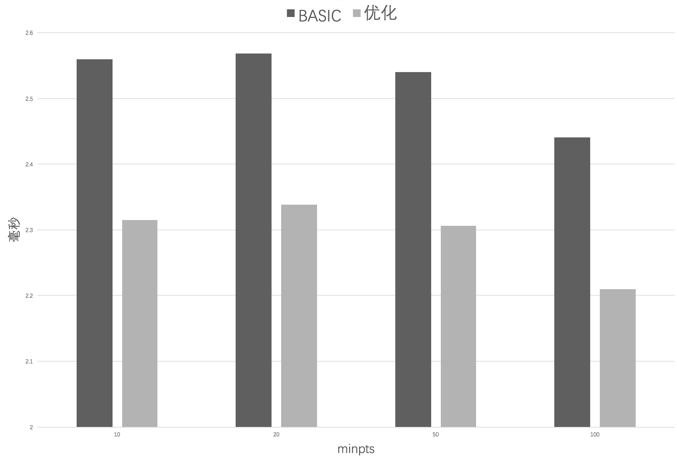
\includegraphics[width=4in]{barchart-change-minpts.png}
    \caption{改变$minpts$}
    \label{change_minpts}
  \end{center}
\end{figure} 

\textbf{3. 改变平衡参数$\alpha$}

\textcolor{red}{\textbf{数据缺失,后续补充。}}

\textbf{4. 改变请求集群数量k}

图\ref{change_k}显示了BASIC算法和改进方法在改变请求集群的k个数量时的性能。由图可知,$k$的变化对于算法性能几乎没有影响。当候选集群未达到$k$个时,算法继续查找集群,阙值为无限大,当集群达到$k$时,算法每次找到一个新的集群,阙值就更新一次并与边界值判断。所以$k$的变化直接带来的是阙值更新的次数,而不会影响得到簇的顺序,也不会带来计算量的显著增长,故对性能的影响较小。 

\begin{figure}[htbp]
  % caption放上面就会显示在图的上方,出现在下面就是出现在图的下方
  % label的位置也有讲究
  \begin{center}
    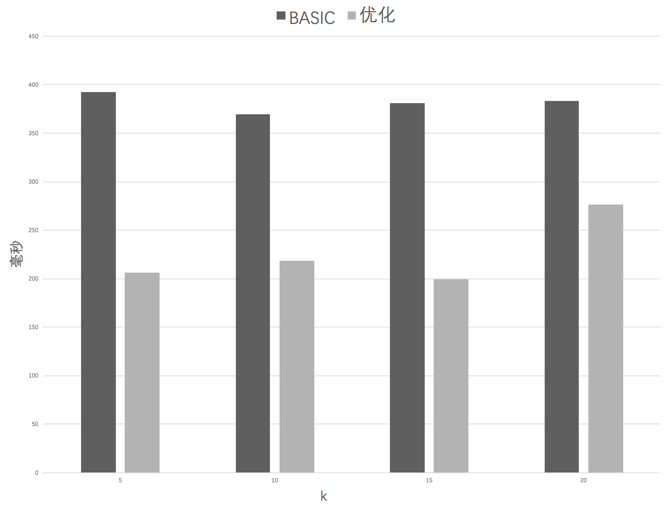
\includegraphics[width=4in]{barchart-change-k.png}
    \caption{改变$k$}
    \label{change_k}
  \end{center}
\end{figure} 

\textbf{5.改变数据集$\left| D \right|$}

图\ref{change_dataset}显示了随着数据集的增大,BASIC算法和改进方法的性能变化。数据集对算法性能的影响是非常直观的,因为数据量直接带来了相关对象的增长,也就提高了计算量,因为而随着数据量的增长,性能表现越差。

\begin{figure}[htbp]
  % caption放上面就会显示在图的上方,出现在下面就是出现在图的下方
  % label的位置也有讲究
  \begin{center}
    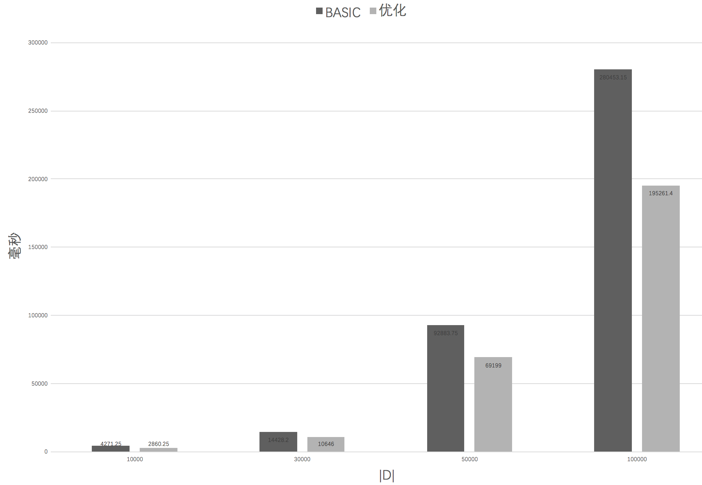
\includegraphics[width=4in]{change-dataset.png}
    \caption{改变数据集}
    \label{change_dataset}
  \end{center}
\end{figure} 
